\pagestyle{empty}

% Tiêu đề đầu trang (Running Header)
\noindent\textbf{304}\qquad\textbf{\textsf{CHƯƠNG 4}}\quad\textsf{CÁC ỨNG DỤNG CỦA ĐẠO HÀM}
\vspace{12pt}

% Cấu hình 2 cột bất đối xứng: Cột lề trái (ghi chú, nhãn hình) và Cột nội dung chính
\setcolumnwidth{4.3cm, 12.8cm}
\setlength{\columnsep}{0.8cm}

\begin{paracol}{2}
% --- CỘT LỀ TRÁI ---
\begin{flushleft}
{\footnotesize\color{black!90}
\noindent Hãy thử vẽ lại đồ thị trong Hình 13 bằng máy tính bỏ túi có chức năng vẽ đồ thị hoặc máy vi tính. Một số máy vẽ được toàn bộ đồ thị, một số chỉ vẽ phần bên phải của trục $y$, và một số chỉ vẽ phần nằm giữa $x = 0$ và $x = 6$. Để xem giải thích, hãy xem Ví dụ 7 trong phần \emph{Máy tính bỏ túi và Máy vi tính vẽ đồ thị} tại \url{www.StewartCalculus.com}.\par
}

\vspace{42pt}
\noindent\textbf{\textsf{HÌNH 13}}
\end{flushleft}

\switchcolumn

% --- CỘT NỘI DUNG CHÍNH ---
\noindent đạo hàm cấp hai, ta vẽ phác đồ thị ở Hình 13. Lưu ý rằng đường cong có các tiếp tuyến thẳng đứng tại $(0, 0)$ và $(6, 0)$ do $|f'(x)| \to \infty$ khi $x \to 0$ và khi $x \to 6$.

\begin{center}
  \vspace{2pt}
  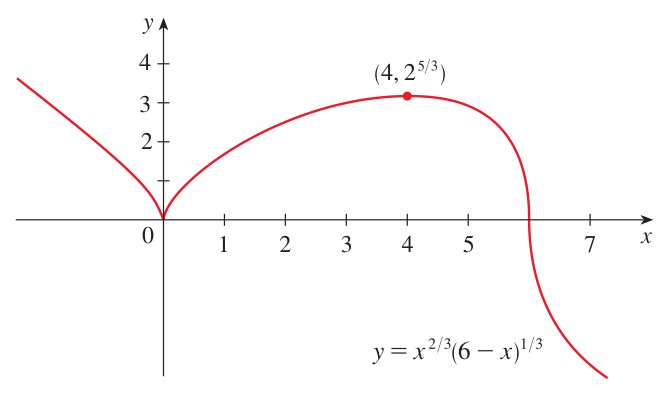
\includegraphics[width=0.72\linewidth]{images/p0339_fig1.png}
\end{center}
\vspace{-12pt}
\hfill\textcolor{stewartblue}{\rule{1.2ex}{1.2ex}}\par
\vspace{14pt}

\noindent{\color{stewartblue}\textbf{\textsf{VÍ DỤ 8}}}\quad Sử dụng các đạo hàm cấp một và cấp hai của $f(x) = e^{1/x}$, cùng với các đường tiệm cận, để vẽ phác đồ thị của hàm số.\par
\vspace{7pt}

\noindent{\color{stewartblue}\textbf{\textsf{LỜI GIẢI}}}\quad Lưu ý rằng tập xác định của $f$ là $\{x \mid x \neq 0\}$, vì vậy ta kiểm tra các đường tiệm cận đứng bằng cách tính các giới hạn một bên khi $x \to 0$. Khi $x \to 0^+$, ta biết rằng $t = 1/x \to \infty$, do đó
\[
\lim_{x \to 0^+} e^{1/x} = \lim_{t \to \infty} e^t = \infty
\]
và điều này cho thấy $x = 0$ là một đường tiệm cận đứng. Khi $x \to 0^-$, ta có $t = 1/x \to -\infty$, vì vậy
\[
\lim_{x \to 0^-} e^{1/x} = \lim_{t \to -\infty} e^t = 0
\]
Khi $x \to \pm\infty$, ta có $1/x \to 0$ và do đó
\[
\lim_{x \to \pm\infty} e^{1/x} = e^0 = 1
\]
Điều này chứng tỏ rằng $y = 1$ là một đường tiệm cận ngang (về cả hai phía trái và phải).\par
\vspace{4pt}

Bây giờ ta hãy tính đạo hàm. Quy tắc chuỗi cho ta
\[
f'(x) = -\frac{e^{1/x}}{x^2}
\]
Vì $e^{1/x} > 0$ và $x^2 > 0$ với mọi $x \neq 0$, nên ta có $f'(x) < 0$ với mọi $x \neq 0$. Do đó $f$ nghịch biến trên $(-\infty, 0)$ và trên $(0, \infty)$. Hàm số không có số tới hạn nào, vì vậy không có giá trị cực đại hay cực tiểu địa phương. Đạo hàm cấp hai là
\[
f''(x) = -\frac{x^2 e^{1/x}(-1/x^2) - e^{1/x}(2x)}{x^4} = \frac{e^{1/x}(2x + 1)}{x^4}
\]
Vì $e^{1/x} > 0$ và $x^4 > 0$, ta có $f''(x) > 0$ khi $x > -\frac{1}{2}$ ($x \neq 0$) và $f''(x) < 0$ khi $x < -\frac{1}{2}$. Do đó đường cong lõm xuống trên $(-\infty, -\frac{1}{2})$ và lõm lên trên $(-\frac{1}{2}, 0)$ và trên $(0, \infty)$. Đồ thị có một điểm uốn là: $(-\frac{1}{2}, e^{-2})$.\par
\vspace{4pt}

Để phác họa đồ thị của $f$, trước tiên ta vẽ đường tiệm cận ngang $y = 1$ (dưới dạng đường nét đứt), cùng với các phần của đường cong ở gần các đường tiệm cận trong một hình vẽ phác sơ bộ [Hình 14(a)]. Các phần này phản ánh thông tin liên quan đến các giới hạn và sự kiện rằng $f$ nghịch biến trên cả $(-\infty, 0)$ và $(0, \infty)$. Lưu ý rằng chúng ta đã chỉ ra $f(x) \to 0$ khi $x \to 0^-$ mặc dù $f(0)$ không tồn tại. Trong Hình 14(b), chúng ta hoàn thành

\end{paracol}

\vfill
\begin{center}
{\fontsize{5.5pt}{6.5pt}\selectfont\color{gray}
Copyright 2021 Cengage Learning. All Rights Reserved. May not be copied, scanned, or duplicated, in whole or in part. WCN 02-200-203\\ 
Editorial review has deemed that any suppressed content does not materially affect the overall learning experience. Cengage Learning reserves the right to remove additional content at any time if subsequent rights restrictions require it.
}
\end{center}
